\documentclass[main.tex]{subfiles}
\pagenumbering{arabic}
\newcommand\chapterlabel{ChMIX-biomoleculesinsolution}\setcounter{figurenewcounter}{0}\setcounter{tablenewcounter}{0}\setcounter{formulanewcounter}{0}
\setcounter{chapter}{4}

\begin{document}



\chapter[Gases  ]{Gases }

\begin{marginfigure}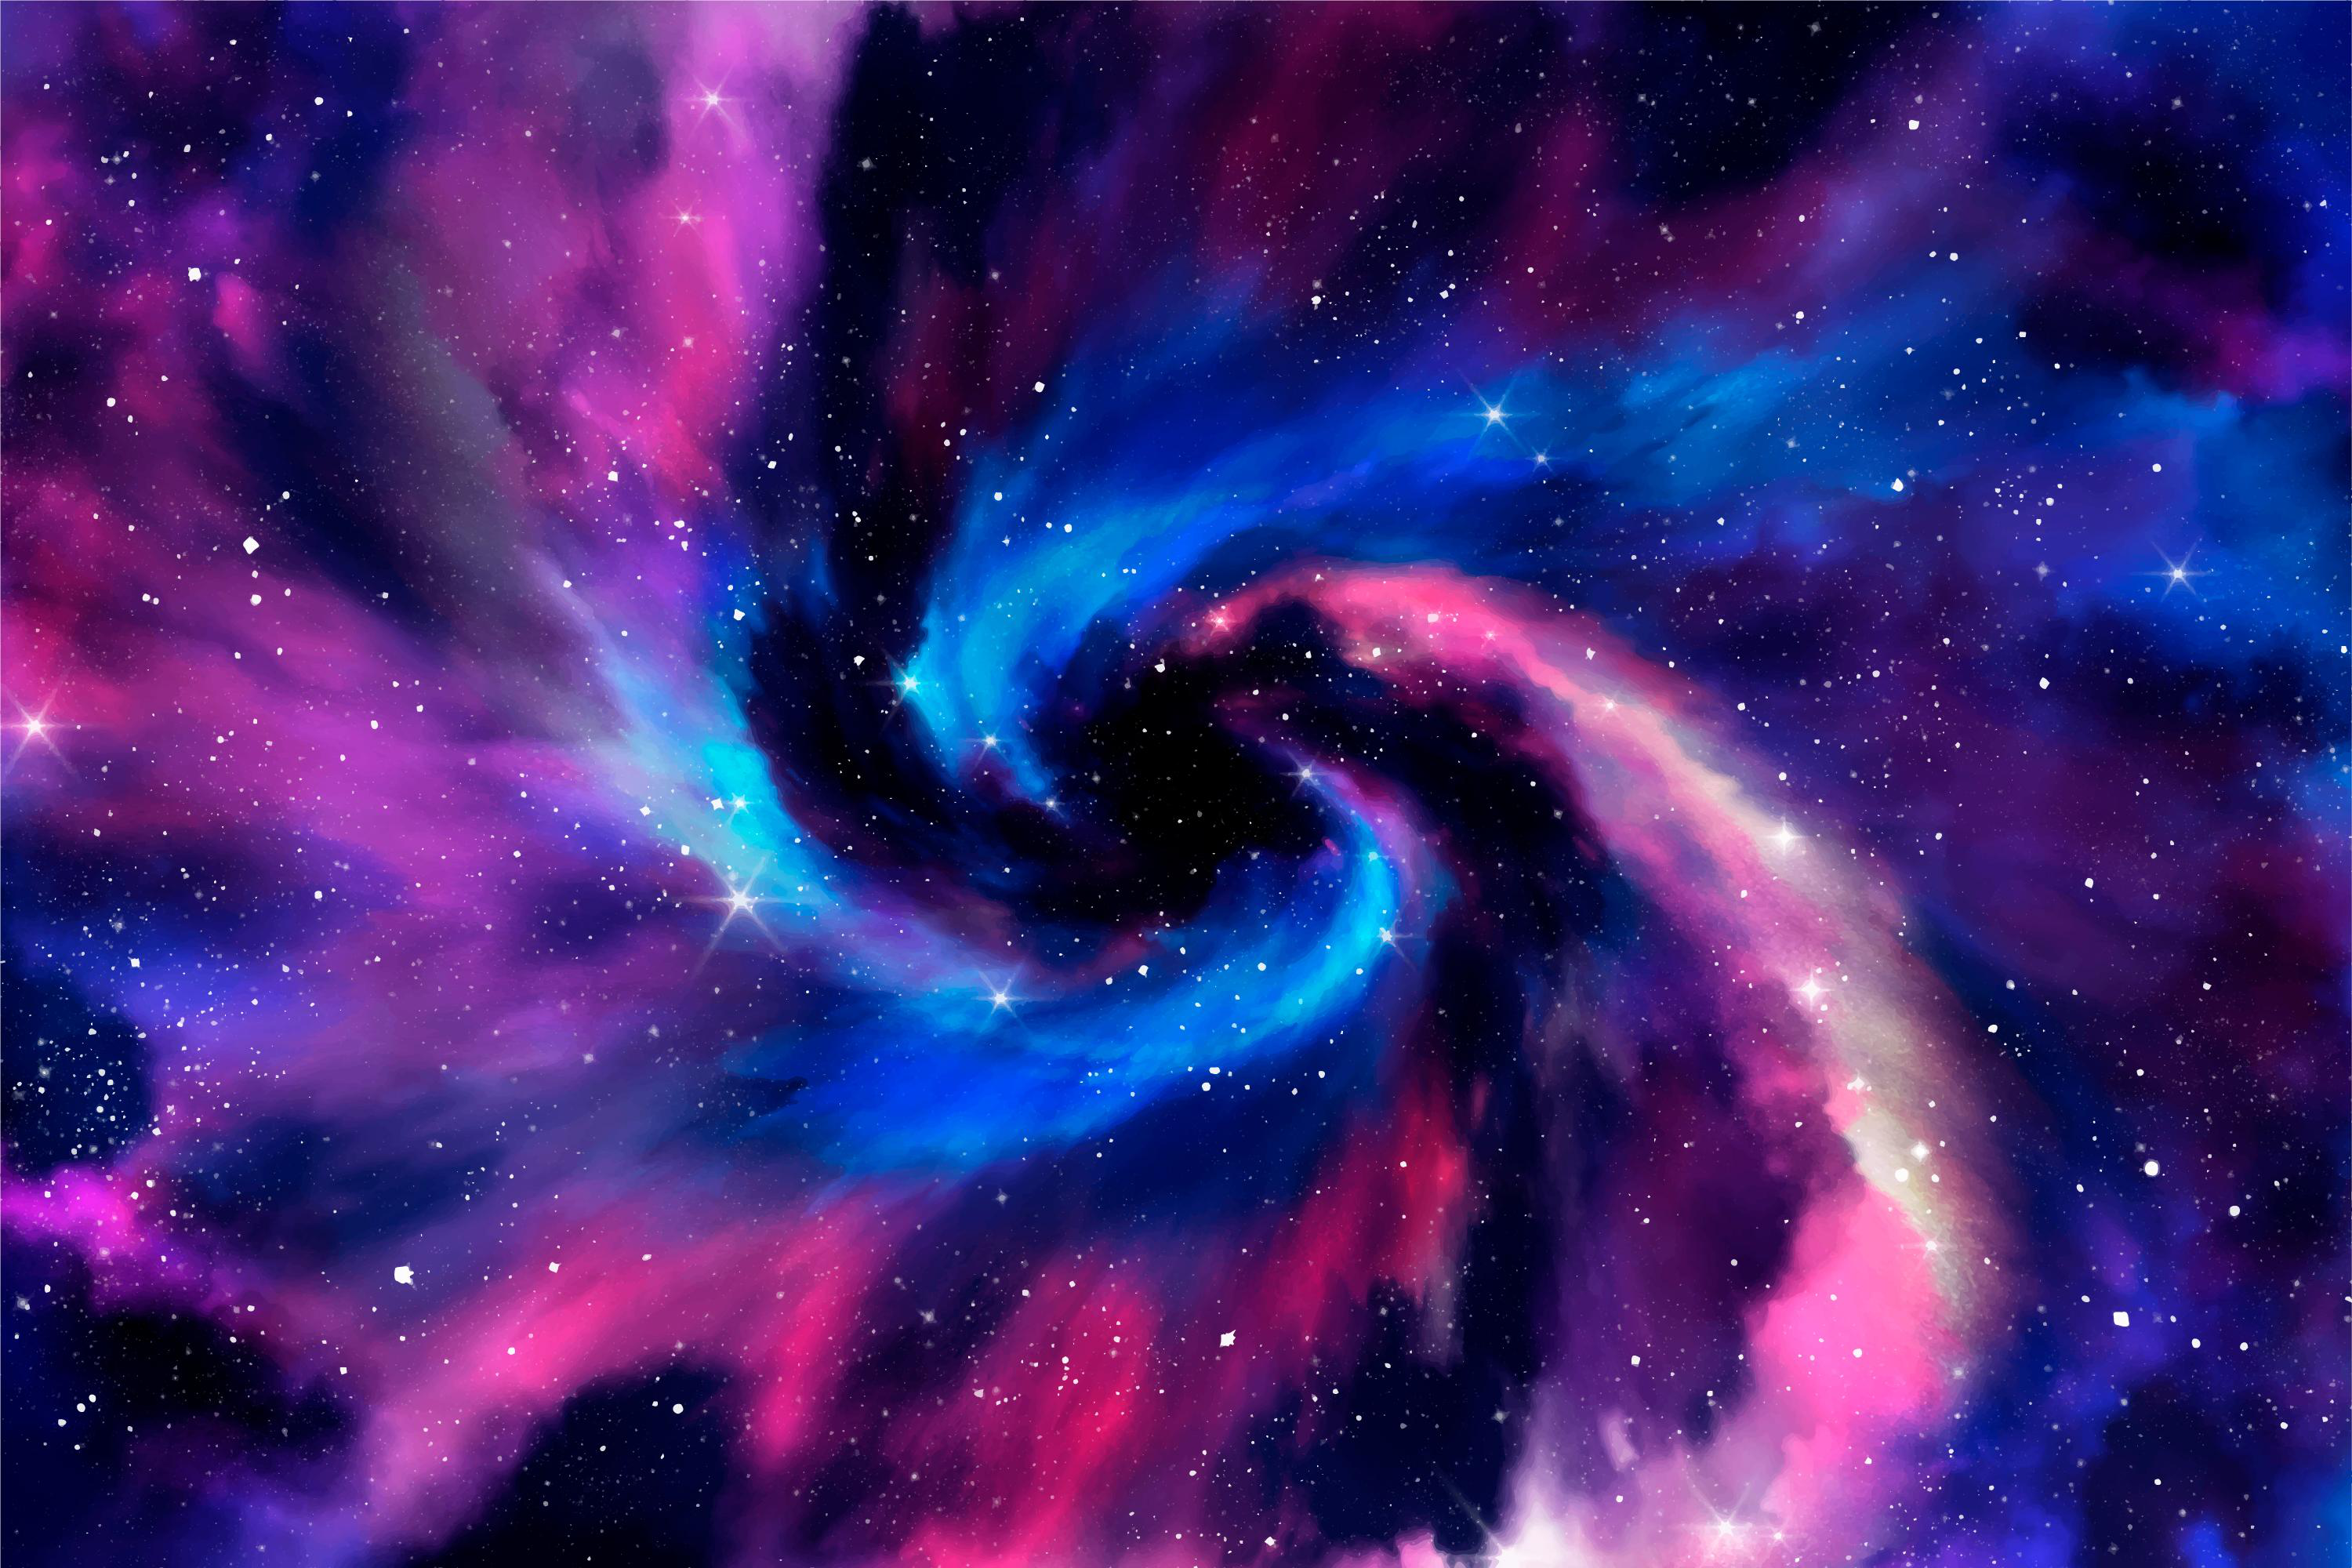
\includegraphics{../Ch-Gas/figure1} \end{marginfigure}\import{../Ch-gas/files/}{ChapterIntro}

\begin{marginfigure}%LEARNING GOALS BOX
\begin{mytcbox}{GOALS}
%
\begin{center}\textcolor{blue}{\faEnvira Chemistry and molecules }\end{center}
\begin{enumerate}[label=\protect\circled{\color{white}\arabic*}]
  \import{../Ch-Gas/files/}{ChapterGoal-Ideal-gas-law}
\end{enumerate}

\begin{center}\textcolor{blue}{\faFlask Acids and bases }\end{center}
\begin{enumerate}[label=\protect\circled{\color{white}\arabic*}]
\import{../Ch-acidbase/files/}{SectionGoal-Blood-as-a-buffer-The-dangerous-change-in-blood-PH}
\end{enumerate}

\begin{center}\textcolor{blue}{\faTint  Electrolytes and solutions }\end{center}
\begin{enumerate}[label=\protect\circled{\color{white}\arabic*}]
\import{../Ch-Gas/files/}{ChapterGoal-Mixtures-of-gases}
\end{enumerate}

\begin{center}\textcolor{blue}{\faFire Reactions and energy} \end{center}
\begin{enumerate}[label=\protect\circled{\color{white}\arabic*}]
 \import{../Ch-mole/files/}{SectionGoal-Chemical-reaction-Balancing-chemical-reactions}
\end{enumerate}

\begin{center}\textcolor{blue}{\faFlash The chemistry of cancer} \end{center}
\begin{enumerate}[label=\protect\circled{\color{white}\arabic*}]
\import{../Ch-nuclear/files/}{SectionGoal-Radioactive-gases:-radon}
	\end{enumerate}
	
\begin{center}\textcolor{blue}{\faFlash Let's calculate} \end{center}
\begin{enumerate}[label=\protect\circled{\color{white}\arabic*}]
\import{../Ch-measurements/files/}{SectionGoal-Using-Conversion-Factors-Square-or-cubic-units}
\import{../Ch-measurements/files/}{SectionGoal-Using-Conversion-Factors-Units-of-volume}
\end{enumerate}
			 				 




\end{mytcbox}
\vspace{1cm}
%\begin{tcolorbox}[enhanced,colback=red!5!white,colframe=black!50!red,boxrule=1pt,
%  arc=0pt,outer arc=0pt,drop heavy lifted shadow]
%\faGears\ 
% \import{../Ch-electrolytes/files/}{ChapterDiscussion}
% \end{tcolorbox}
\end{marginfigure}%LEARNING GOALS BOX






\renewcommand\chapterlabel{Ch-Gas}



\section{\faEnvira Gases and its properties} \import{../\chapterlabel/files/}{SectionIntro-Gases-and-its-properties}
\sloppy \begin{description}
\item[\docfilehook{Gases in the periodic table}{}]  \import{../\chapterlabel/files/}{SubSection-Gases-and-its-properties-Gases-in-the-periodic-table}
\item[\docfilehook{Characteristics of gases}{}]  \import{../\chapterlabel/files/}{SubSection-Gases-and-its-properties-Characteristics-of-gases}
 \item[\docfilehook{Volume, V}{}] \import{../\chapterlabel/files/}{SubSection-Gases-and-its-properties-Volume,-V}
 \item[\docfilehook{Temperature, T}{}]\import{../\chapterlabel/files/}{SubSection-Gases-and-its-properties-Temperature,-T}
 \import{../\chapterlabel/files/}{Figure-Gas-Table}
 \item[\docfilehook{Amount of gas, n}{}] \import{../\chapterlabel/files/}{SubSection-Gases-and-its-properties-Amount-of-gas,-n}
 \import{../\chapterlabel/files/}{SideFigure-Gases}
\item[\docfilehook{Pressure, P}{}] \import{../\chapterlabel/files/}{SubSection-Gases-and-its-properties-Pressure,-P}
\import{../\chapterlabel/problems/}{SampleProblem1}
 \import{../\chapterlabel/files/}{Figure-Pressure}
\end{description}




 \section{\faEnvira Ideal gas law}\import{../\chapterlabel/files/}{SectionIntro-Ideal-gas-law}
\sloppy \begin{description}
 \import{../\chapterlabel/files/}{SubSection-Ideal-gas-law-Ideal-gas-law-in-terms-of-moles}
\import{../\chapterlabel/problems/}{SampleProblem2}
 \import{../\chapterlabel/files/}{SubSection-Ideal-gas-law-Ideal-gas-law-in-terms-of-density}
\import{../\chapterlabel/problems/}{SampleProblem3}
 \import{../\chapterlabel/files/}{SubSection-Ideal-gas-law-STP-conditions}
\import{../\chapterlabel/problems/}{SampleProblem4}
\end{description}


 \section{\faEnvira Change of gas properties}\import{../\chapterlabel/files/}{SectionIntro-Change-of-gas-properties}
\sloppy \begin{description}
\item[\docfilehook{Solving problems with an initial and final state}{}]  \import{../\chapterlabel/files/}{SubSection-Change-of-gas-properties-Solving-problems-with-an-initial-and-final-state}
\import{../\chapterlabel/problems/}{SampleProblem5}
\item[\docfilehook{Pressure-Volume change}{}] \import{../\chapterlabel/files/}{SubSection-Change-of-gas-properties-Pressure-Volume-change}
 \item[\docfilehook{Volume-Moles change}{}] \import{../\chapterlabel/files/}{SubSection-Change-of-gas-properties-Volume-Moles-change}
\item[\docfilehook{Relating the different variables of a gas}{}]  \import{../\chapterlabel/files/}{SubSection-Change-of-gas-properties-Relating-the-different-variables-of-a-gas}
\end{description}



%  \section{\faEnvira Kinetic molecular theory of gases }\import{../\chapterlabel/files/}{SectionIntro-the-kinetic-molecular-theory-of-gases}
% \sloppy 
%\begin{description}
% \item[\docfilehook{Kinetic theory of gases}{}] \import{../\chapterlabel/files/}{SubSection-Real-gases-and-the-kinetic-molecular-theory-of-gases-Kinetic-theory-of-gases}
%\import{../\chapterlabel/problems/}{SampleProblem11}
%\end{description}
 



 
 \section{\faTint Mixtures of gases  }\import{../\chapterlabel/files/}{SectionIntro-Mixtures-of-gases-and-gas-stoichiometry}
\sloppy 
\begin{description}
 \item[\docfilehook{Partial and total pressure}{}] 
\import{../\chapterlabel/files/}{SubSection-Mixtures-of-gases-and-gas-stoichiometry-Partial-and-total-pressure}
\import{../\chapterlabel/problems/}{SampleProblem7}
 \import{../\chapterlabel/files/}{Figure-Partial-Pressure}
\item[\docfilehook{Partial pressure of a gas in a mixture}{ }]  \import{../\chapterlabel/files/}{SubSection-Mixtures-of-gases-and-gas-stoichiometry-Partial-pressure-of-a-gas-in-a-mixture}
\item[\docfilehook{Mole fraction}{}]  \import{../\chapterlabel/files/}{SubSection-Mixtures-of-gases-and-gas-stoichiometry-Mole-fraction}
\import{../\chapterlabel/problems/}{SampleProblem8}
\end{description}





 



\renewcommand\chapterlabel{Ch-naming}
\section{\faEnvira Covalent compounds}
\import{../\chapterlabel/files/}{SectionIntro-Covalent-compounds}
\sloppy \begin{description}
\import{../\chapterlabel/files/}{Subsection-Covalent-compounds-Covalent-naming}
 \import{../\chapterlabel/files/}{Table-Covalent-prefixes}	
\import{../\chapterlabel/problems/}{SampleProblem5}
\import{../\chapterlabel/files/}{Subsection-Covalent-compounds-Properties-of-covalent-compounds}
\import{../\chapterlabel/files/}{Subsection-Covalent-compounds-The-covalent-bond}
\end{description}



\renewcommand\chapterlabel{Ch-nuclear}
\section{\faFlash Radioactive gases: radon}
\import{../\chapterlabel/files/}{SectionIntro-Radioactive-gases:-radon}

\renewcommand\chapterlabel{Ch-acidbase}

\section{\color{blue!30!black}{\faFlask Blood as a buffer}}\import{../\chapterlabel/files/}{SectionIntro-Blood-as-a-buffer}
\sloppy
\begin{description}
\item[\docfilehook{ Carbon dioxide is an acid}{}] \import{../\chapterlabel/files/}{SubSection-Blood-as-a-buffer-Carbon-dioxide-is-an-acid}
\item[\docfilehook{ The dangerous change in blood PH}{}] 
\import{../\chapterlabel/files/}{SubSection-Blood-as-a-buffer-The-dangerous-change-in-blood-PH}
  \import{../\chapterlabel/files/}{Figure-Alkalosis-and-PH}
\item[\docfilehook{ Alkalosis and carbon dioxide}{}] 
\import{../\chapterlabel/files/}{SubSection-Blood-as-a-buffer-Alkalosis-and-carbon-dioxide}
   \import{../\chapterlabel/problems/}{SampleProblem20}
 \end{description}

\renewcommand\chapterlabel{Ch-mole}
\section{\faFire Chemical reactions}
\import{../\chapterlabel/files/}{SectionIntro-Chemical-reaction}
\sloppy\begin{description}
\import{../\chapterlabel/files/}{SubSection-Chemical-reaction-Simple-chemical-reactions}
\import{../\chapterlabel/files/}{SubSection-Chemical-reaction-Reading-a-chemical-reaction}
\import{../\chapterlabel/files/}{SubSection-Chemical-reaction-Balanced-chemical-reactions}
\import{../\chapterlabel/problems/}{SampleProblem5}
\end{description}

\renewcommand\chapterlabel{Ch-measurements}
\section{\faGears Square units and units of volume}
\sloppy\begin{description}
\item[\docfilehook{Square or cubic units}{}]\import{../\chapterlabel/files/}{SubSection-Using-Conversion-Factors-Square-or-cubic-units}
\import{../\chapterlabel/problems/}{SampleProblem5}
\item[\docfilehook{Units of volume}{}]\import{../\chapterlabel/files/}{SubSection-Using-Conversion-Factors-Units-of-volume}
\import{../\chapterlabel/problems/}{SampleProblem6}
\end{description}

 






\end{document}
 
